\documentclass[8pt,a4paper,titlepage]{article}

% Set document dimensions
\usepackage[paper=a4paper,top=2cm,left=2cm,right=2cm,bottom=2cm,includefoot]{geometry}

% For todo notes
\usepackage{todonotes} 

% Set czech font
\usepackage[T1]{fontenc}
\usepackage[utf8]{inputenc}
\usepackage[czech]{babel}

% Set packages for including images
\usepackage{graphicx}
\usepackage{svg}
\graphicspath{ {src/assets/} }
\usepackage{pdfpages}
\usepackage{color} % barvy
\usepackage{xcolor} % vytváření barev

% Include pseudo-algorithm to latex document
\usepackage{algorithm2e}

% Colour our links, remove weird boxes
\usepackage[colorlinks,linkcolor={black},citecolor={blue!80!black},urlcolor={blue!80!black}]{hyperref}

% Stop indentation on new paragraphs
\usepackage[parfill]{parskip}

% Give us the Capital H that we all know and love
\usepackage{float}

% Tone down the line spacing after section titles

\usepackage{titlesec}

% Cool maths printing
\usepackage{amsmath}

% latex magic
\usepackage{newverbs}

\usepackage{enumitem}

% Packages for including source code to latex document
\usepackage{listings}

\definecolor{codeprimary}{HTML}{3300CC}
\colorlet{keywordstyle}{codeprimary!50!black}

\lstset{
	escapeinside={/*@}{@*/}, language=C,
	basicstyle=\fontsize{12}{14}\selectfont,
	numbers=left,numbersep=2pt,xleftmargin=2pt,frame=tb,
    columns=fullflexible,showstringspaces=false,tabsize=4,
    keepspaces=true,showtabs=false,showspaces=false,
    backgroundcolor=\color{white}, morekeywords={inline,public,
    class,private,protected,struct},captionpos=t,lineskip=-0.4em,
	aboveskip=10pt, extendedchars=true, breaklines=true,
	prebreak = \raisebox{0ex}[0ex][0ex]{\ensuremath{\hookleftarrow}},
	keywordstyle=\color[rgb]{0,0,1},
	commentstyle=\color[rgb]{0.133,0.545,0.133},
	stringstyle=\color[rgb]{0.627,0.126,0.941}
}

% \ic for inline code
\makeatletter
\newcommand\ic[1][green]{%
    \@testopt{\@ic{#1}}{-#1}% Handle second optional argument
}
\def\@ic#1[#2]{%
    \Collectverb{\@@ic{#1}{#2}}%
}
\def\@@ic#1#2#3{%
    {\lstinline[basicstyle=\ttfamily\color{codeprimary},breaklines=true]|#3|}%
}
\newcommand{\icmacro}[1]{{\lstinline[basicstyle=\ttfamily\color{codeprimary},breaklines=true]|#1|}}
\makeatother

\usepackage{pdflscape}
% For table of contents
\usepackage[tocflat]{tocstyle}
\usetocstyle{standard}
\usepackage{blindtext}
% Redefinition of ToC command to get centered heading
\makeatletter
\renewcommand\tableofcontents{%
  \null\hfill\textbf{\Large\contentsname}\hfill\null\par
  \@mkboth{\MakeUppercase\contentsname}{\MakeUppercase\contentsname}%
  \@starttoc{toc}%
}
\makeatother

% Body of document
\begin{document}
	\begin{titlepage}
	\centering

	{\fontsize{20pt}{15pt}\bfseries 
		VYSOKÉ UČENÍ TECHNICKÉ V~BRNĚ\\
		\vspace{8pt}
		Fakulta informačních technologií
	}

	\vspace*{64pt}

	\includegraphics{./build/output.pdf}
	\vspace*{22pt}

	{\Large Dokumentace k projektu do předmětů IFJ a IAL\\}
	\vspace*{4pt}
	{\LARGE \bfseries Implementace interpretu jazyka IFJ17\\}
	\vspace*{62pt}
	{\Large \bfseries Tým XX, varianta x/x/XX\\}
	\vspace*{42pt}
	{\Large \today}

	\vspace*{64pt}
	{\Large \bfseries Autoři\\}
	\vspace*{8pt}
	\begin{tabular}{ l c r }
	  Josef Kolář & \textit{xkolar71} & 69 \% \\
	  Son Hai Nguyen & \textit{xnguye16} & 69 \% \\
	  Martin Kobelka & \textit{xkobel02} & 69 \% \\
	  Xxxxxxxx Xxxxx & \textit{xxxxxxDD} & 69 \% \\
	  Xxxx Xxxxxxxxx & \textit{xxxxxxDD} & 69 \% \\
	\end{tabular}\\
	\vspace*{32pt}
	{\Large \bfseries Seznam rozšíření\\}
	\vspace*{8pt}
	Tato, všechna, rozšíření, jsme, implementovali\\
	\vspace*{64pt}

\end{titlepage}
	 
\tableofcontents
\newpage
	\section{Úvod}
Následující dokument popisuje způsob implementace kompilátoru z~jazyka IFJ17 do mezikódu
IFJcode17 ve variantě 2. Jedná se o~projekt, který byl vyprácován podle zadání do předmětů IFJ a IAL na Fakultě
informačních technologí Vysokého učení technického v~Brně. Dokumentuje způsob řešení, dekompozici překladače na jednotlivé moduly, popis použitých algoritmů a datových struktur a  v závěru je zmíněn také způsob práce v~týmu.

\section{Teoretický rozbor}
Naším úkolem bylo implementovat překladač jazyka IFJ17 (který je modifikovanou podmnožinou jazyka známého jako \mbox{FREEBASIC})
do mezikódu IFJcode17. Program čte zdrojový kód ze standardního vstupu a v~případě překladu bez chyby generuje cílový
kód. V~případě chyby je navrácen odpovídající chybový kód a vytisknuta informace o~typu chyby. Varianta 2 specifikuje
zadání na užití tabulky s~rozptýlenými položkami při implementaci tabulky symbolů.

Pro běh překladače byl použit tzv. \textbf{Syntaxí řízený překlad}, což předurčuje syntaktický analyzátor k~řízení činnosti
celého překladače. SA tedy získává vstupní tokeny a kontroluje, zda tvoří řetězec generovaný
LL gramatikou, spouští sémantické kontroly a řídí konstrukci kódu.
Optimalizátor poté pracuje po dokončení syntaxí řízeného překladu nad vygenerovaným kódem.

Implementace překladače se nám tedy dělí na následující moduly:
\begin{itemize}
    \item Lexikální analyzátor
    \item Syntaktický analyzátor
    \item Sémantický analyzátor,
    \item Generátor cílového kódu
    \item Optimalizátor kódu
\end{itemize}

Jelikož výstupem překladu je jistá forma mezikódu, používáme metodu generování tohoto kódu přímo ze syntaktické analýzy \textbf{bez generování abstraktního syntaktického stromu} nebo zásobníkového kódu.

Propojení jednotlivých komponent naznačuje následující schéma:
\vspace*{4px}
\begin{figure}[htbp]
	\centering
	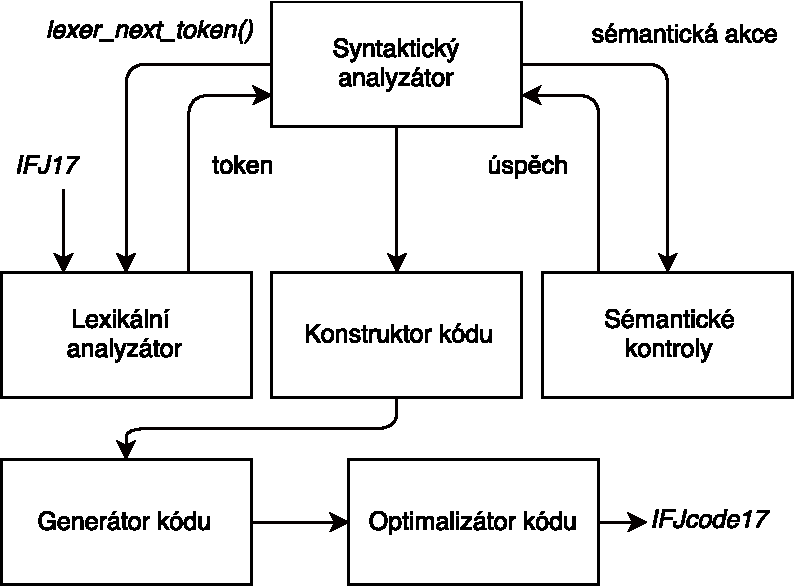
\includegraphics[width=0.65\textwidth, angle=0]{src/assets/structure.pdf}
\end{figure}
	\subsection{Lexikální analýza}
\label{subsec:lexer}
Úlohou Lexikálního analyzátoru je rozpoznávat jazykové lexémy a reprezentovat
je jako tokeny.

Lexikální analyzátor je implementací deterministického konečného
automatu. Jediný nedeterministický případ nastává tehdy, když má automat načítat znak ve tvatu $\backslash$ddd.
Případ je vyřešen implementací interního čítače počtu číslic.

Lexikální analyzátor je rozdělen do tří modulů: \ic|lexer.c|, \ic|lexer_fsm.c| a \ic|token.c|
. Modul \ic|token.c| obsahuje implementaci abstraktního datového typu token. Modul \ic|lexer_fsm.c|
obsahuje implementaci deterministického konečného automatu. Modul \ic|lexer.c| poskytuje funkci
\ic|lexer_next_token|, která řídí činnost deterministického konečného automatu a
která vrací další token.

\vspace*{16px}
\begin{figure}[htbp]
    \centering
    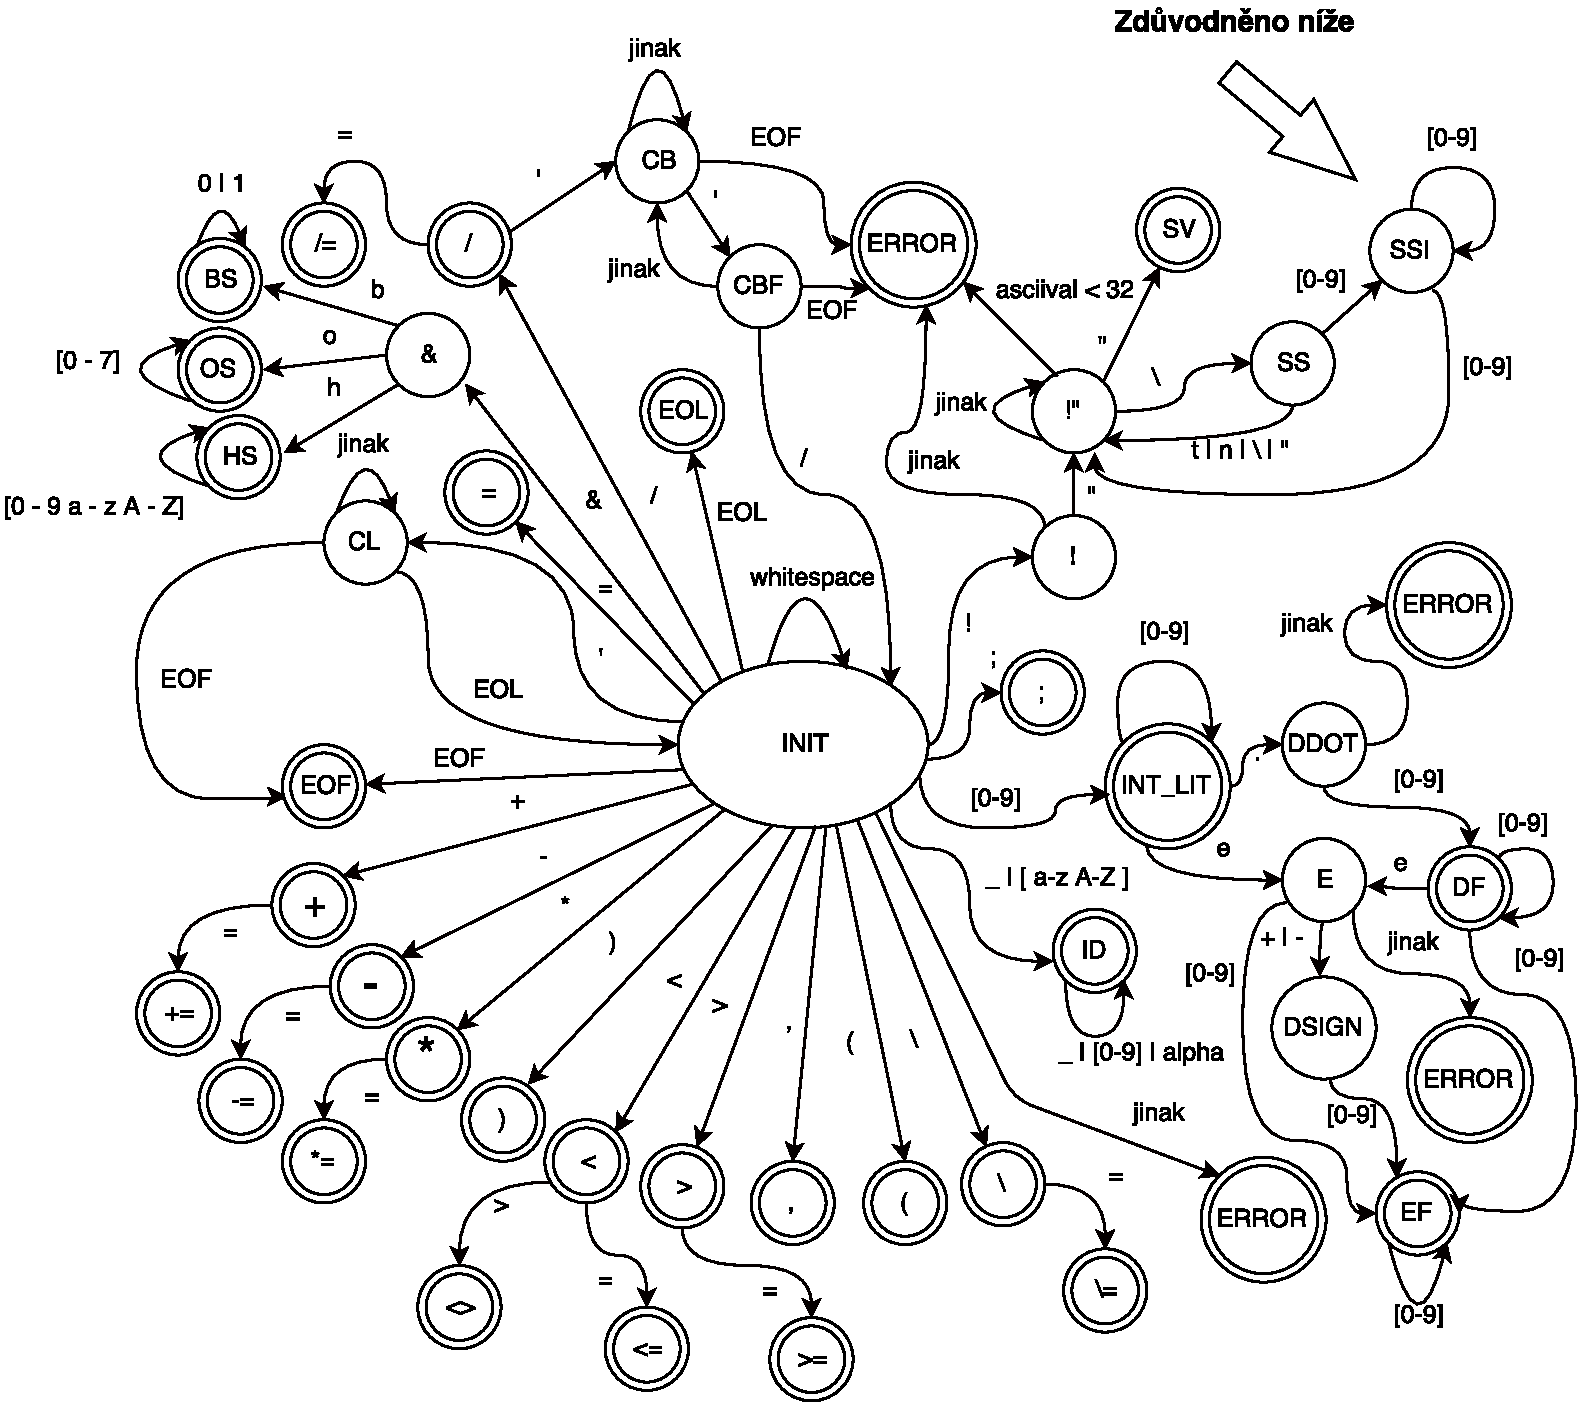
\includegraphics[width=1\textwidth, angle=0]{src/assets/automat.pdf}
\end{figure}

\subsection{Synataktická analýza}
Syntaxí řízený překlad je naimplementován v modulu \ic|parser.c|, pro syntaktickou analýzu programu jako takového je
použita SA shoda dolů, konkrétně metoda rekurzivního sestupu. Pro každé pravidlo z LL gramatiky existuje v tomto
modulu funkce realizující toto pravidlo.

Pro snažší zápis v jazyce C byl implementován poloautomatický systém generování funkcí reprezentující tato pravidla za pomocí maker.
Makra konkrétní pravidlo zavolají a zkontrolují jeho splnění. Pro kontrolu terminálu bylo naimplemntováno makro
\ic|CHECK_TOKEN(TOKEN_TYPE)|,
Pro zavolání pravidla bylo naimplementováno pravidlo \ic|CALL_RULE(NAME_OF_RULE);|.
Pro podmínečná volání pravidel poté makro ve stylu
\ic|CHECK_RULE(token_type == TOKEN_TYPE, NAME_OF_RULE, REWIND_AND_SUCCESS)| - Pri použití se zavolá pravidlo
\ic|NAME_OF_RULE| v případě, že je následující token typu \ic|TOKEN_TYPE| a jestliže bylo úspěšné, další načtený
token navrátí zpět a prohlásí volání za úspěšné.

Všechny pravidla pracují nad strukturou \ic|Parser|, která zapouzdřuje základní komponenty pro syntaxí řízený překlad.
Jedná se především od struktury \ic!ParserSemantic!, \ic!CodeConstructor! a \ic!Lexer!. První zmíněná zajištuje sémantické
kontroly programu; uchovává \emph{registr symbolů}, dočasné proměnné, pravidla pro implicitní konverze datových typů či
aktuální scénář SA. Konstruktor kódu je poté popsán v příslušné sekci \ref{subsec:code-constructor}, Lexer v sekci
\ref{subsec:lexer}.

Pro analýzu výrazů není analýza shora dolů příliš vhodná, proto byla
použita metoda zdola nahoru v našem případě založená na precedenční
syntaktické analýza implementovaná v souboru \ic|parser_expr.c|.

Přepínání mezi metodami je realizováno následujícím mechanismem. Na celý program je použita funkce \ic|parser_parse|
z modulu \ic|parser.c|. V případě že je jako neterminál očekáván výraz, je volána funkce \ic|parser_parse_expr|
z modulu \ic|parser_expr.c|, která provede precedenční syntaktickou analýzu výrazu.

\subsubsection{Gramatika}

\begin{enumerate}
\item <prog> $\rightarrow$ <body> <eols> EOF
\item <body> $\rightarrow$ <definitions> <scope> <shared\_variables\_declarations>
\item <body> $\rightarrow$ <definitions> <statement\_scope>

\item <definitions> $\rightarrow$ <eols> <definition> <definitions>
\item <definitions> $\rightarrow$ <eols> E

\item <definition> $\rightarrow$ <function\_declaration>
\item <definition> $\rightarrow$ <function\_definition>
\item <definition> $\rightarrow$ <shared\_variable\_declaration>

\item <function\_definition> $\rightarrow$ <function\_header> EOL <eols> <statements> END FUNCTION
\item <function\_declaration> $\rightarrow$ DECLARE <function\_header> EOL <eols>

\item <function\_header> $\rightarrow$ FUNCTION IDENTIFIER (<function\_params>) AS <type>

\item <function\_params> $\rightarrow$ E
\item <function\_params> $\rightarrow$ <function\_param> <function\_n\_param>

\item <function\_n\_param> $\rightarrow$ E
\item <function\_n\_param> $\rightarrow$ <function\_param> <function\_n\_param>

\item <function\_param> $\rightarrow$ IDENTIFIER AS <type>


\item <type> $\rightarrow$ INTEGER
\item <type> $\rightarrow$ BOOLEAN
\item <type> $\rightarrow$ STRING
\item <type> $\rightarrow$ DOUBLE

\item <statements> $\rightarrow$ E
\item <statements> $\rightarrow$ <statement\_single> EOL <eols> <statements>


\item <statement\_single> $\rightarrow$ <identifier\_assignment>
\item <statement\_single> $\rightarrow$ <input>
\item <statement\_single> $\rightarrow$ <return>
\item <statement\_single> $\rightarrow$ <print>
\item <statement\_single> $\rightarrow$ <condition>
\item <statement\_single> $\rightarrow$ <while\_>
\item <statement\_single> $\rightarrow$ <variable\_declaration>
\item <statement\_single> $\rightarrow$ <static\_variable\_declaration>
\item <statement\_single> $\rightarrow$ <scope>

\item <variable\_declaration> $\rightarrow$ DIM IDENTIFIER AS <type> <declaration\_assignment>
\item <declaration\_assignment> $\rightarrow$ E
\item <declaration\_assignment> $\rightarrow$ <assignment>

\item <shared\_variables\_declarations> $\rightarrow$ E
\item <shared\_variables\_declarations> $\rightarrow$ <shared\_variable\_declaration>
\item <shared\_variable\_declaration> $\rightarrow$ DIM SHARED IDENTIFIER AS <type> <declaration\_assignment>

\item <static\_variable\_declaration> $\rightarrow$ STATIC IDENTIFIER AS <type> <declaration\_assignment>

\item <return> $\rightarrow$ RETURN <expr>

\item <assignment> $\rightarrow$ <modify> <expression>
\item <modify> $\rightarrow$ +=
\item <modify> $\rightarrow$ -=
\item <modify> $\rightarrow$ *=
\item <modify> $\rightarrow$ /=
\item <modify> $\rightarrow$ $\backslash$=

\item <print> $\rightarrow$ PRINT <print\_expression> <print\_expressions>
\item <print\_expressions> $\rightarrow$ E
\item <print\_expressions> $\rightarrow$ <print\_expression> <print\_expressions>
\item <print\_expression> $\rightarrow$ <expression> SEMICOLON

\item <while\_> $\rightarrow$ DO WHILE <expression> EOL <eols> <cycle\_statements> LOOP

\item <input> $\rightarrow$ INPUT IDENTIFIER

\item <condition> -> IF <expr> THEN EOL <eols> <statements>
\item <condition\_elseif> <condition\_else> END IF
\item <condition\_elseif> -> E
\item <condition\_elseif> -> ELSEIF <expr> THEN EOL <statements> <condition\_elseif>

\item <condition\_else> -> E
\item <condition\_else> -> ELSE EOL <eols> <statements>

\item <eols> $\rightarrow$ E
\item <eols> $\rightarrow$ EOL <eols>

\end{enumerate}
\newpage
\subsection{Precedenční analýza výrazů}
Precedenční analýza je řízena precedenční tabulkou, kterou se vyhodnocuje pořadí zpracování tokenů. \ref{table:prec}
\ic|parser_expr_prec_table_data.c|. V tabulce se nachází jak binární, tak i unární mínus. 
Lexikální analyzátor nám ovšem poskytuje pouze jeden token mínus a proto se unární a binární mínus 
musí vyhodnotit podle kontextu. Precedenční analýza využívá se obousměrně vázaného seznamu, do kterého se ukládají terminály, 
precedenční symboly a neterminály. Pomocí redukčních pravidel, která jsou vypsána v příloze, se postupně výraz redukuje. 
Jelikož překladač je založen na přímém překladu, tak při redukování pomocí pravidel konstruktor kódu rovnou generuje kód programu.

\subsubsection{Redukční pravidla}

\begin{table}[htbp]
\centering
\label{Redukční pravidla}
\begin{tabular}{lll}
    $E \to i$ &  $E \to (E)$ & $E \to (E)$ \\
    $E \to (E)$ & $E \to i()$ & $E \to i(E)$\\
    $E \to i(E, E)$ & $E \to i(E, E, ...)$ &  $E \to E + E$\\
    $E \to E - E$ & $E \to E ~ / ~ E$ & $E \to E ~ \backslash ~ E$\\
    $E \to - E$ &  $E \to E = E$ & $E \to E <> E$\\
    $E \to E > E$ & $E \to E >= E$ & $E \to E < E$\\
    $E \to E <= E$ & $E \to NOT ~ E$ & $E \to E ~ AND ~ E$\\
    $E \to E ~ OR ~ E$ & & \\
\end{tabular}
\end{table}


\begin{table}[htbp]
\label{table:prec}
\centering
\caption{Precedenční tabulka}
\label{precedencni-tabulka}
\begin{tabular}{|l|l|l|l|l|l|l|l|l|l|l|l|l|l|l|l|l|l|l|l|l|}
\hline
& $un -$ & $*$ & $/$ & $\backslash$ & $+$ & $-$ & $=$ & $<>$ & $<$ & $<=$ & $>=$ & $>$ & $NOT$ & $AND$ & $OR$ & $($ & $)$ & $,$ & $i$ & \$ \\ \hline
$un -$ &$<$&$>$&$>$&$>$&$>$&$>$&$>$&$>$&$>$&$>$&$>$&$>$& x &$>$&$>$&$<$&$>$& x &$<$&$>$\\ \hline
$*$ &$<$&$>$&$>$&$>$&$>$&$>$&$>$&$>$&$>$&$>$&$>$&$>$&$<$&$>$&$>$&$<$&$>$&$>$&$<$&$>$\\ \hline
$/$ &$<$&$>$&$>$&$>$&$>$&$>$&$>$&$>$&$>$&$>$&$>$&$>$&$<$&$>$&$>$&$<$&$>$&$>$&$<$&$>$\\ \hline
$\backslash$ &$<$&$<$&$<$&$>$&$>$&$>$&$>$&$>$&$>$&$>$&$>$&$>$&$<$&$>$&$>$&$<$&$>$&$>$&$<$&$>$\\ \hline
$+$ &$<$&$<$&$<$&$<$&$>$&$>$&$>$&$>$&$>$&$>$&$>$&$>$&$<$&$>$&$>$&$<$&$>$&$>$&$<$&$>$\\ \hline
$-$ &$<$&$<$&$<$&$<$&$>$&$>$&$>$&$>$&$>$&$>$&$>$&$>$&$<$&$>$&$>$&$<$&$>$&$>$&$<$&$>$\\ \hline
$=$ &$<$&$<$&$<$&$<$&$<$&$<$&$>$&$>$&$>$&$>$&$>$&$>$&$<$&$>$&$>$&$<$&$>$&$>$&$<$&$>$\\ \hline
$<>$ &$<$&$<$&$<$&$<$&$<$&$<$&$>$&$>$&$>$&$>$&$>$&$>$&$<$&$>$&$>$&$<$&$>$&$>$&$<$&$>$\\ \hline
$<$ &$<$&$<$&$<$&$<$&$<$&$<$&$>$&$>$&$>$&$>$&$>$&$>$&$<$&$>$&$>$&$<$&$>$&$>$&$<$&$>$\\ \hline
$<=$ &$<$&$<$&$<$&$<$&$<$&$<$&$>$&$>$&$>$&$>$&$>$&$>$&$<$&$>$&$>$&$<$&$>$&$>$&$<$&$>$\\ \hline
$>=$ &$<$&$<$&$<$&$<$&$<$&$<$&$>$&$>$&$>$&$>$&$>$&$>$&$<$&$>$&$>$&$<$&$>$&$>$&$<$&$>$\\ \hline
$>$ &$<$&$<$&$<$&$<$&$<$&$<$&$>$&$>$&$>$&$>$&$>$&$>$&$<$&$>$&$>$&$<$&$>$&$>$&$<$&$>$\\ \hline
$NOT$ & x &$>$&$>$&$>$&$>$&$>$&$>$&$>$&$>$&$>$&$>$&$>$&$<$&$>$&$>$&$<$&$>$& x &$<$&$>$\\ \hline
$AND$ &$<$&$<$&$<$&$<$&$<$&$<$&$<$&$<$&$<$&$<$&$<$&$<$&$<$&$>$&$>$&$<$&$>$&$>$&$<$&$>$\\ \hline
$OR$ &$<$&$<$&$<$&$<$&$<$&$<$&$<$&$<$&$<$&$<$&$<$&$<$&$<$&$<$&$>$&$<$&$>$&$>$&$<$&$>$\\ \hline
$($ &$<$&$<$&$<$&$<$&$<$&$<$&$<$&$<$&$<$&$<$&$<$&$<$&$<$&$<$&$<$&$<$& = & = &$<$& x \\ \hline
$)$ &$>$&$>$&$>$&$>$&$>$&$>$&$>$&$>$&$>$&$>$&$>$&$>$&$>$&$>$&$>$& x &$>$&$>$& x &$>$\\ \hline
$,$ &$<$&$<$&$<$&$<$&$<$&$<$&$<$&$<$&$<$&$<$&$<$&$<$&$<$&$<$&$<$&$<$& = & = &$<$& x \\ \hline
$i$ & x &$>$&$>$&$>$&$>$&$>$&$>$&$>$&$>$&$>$&$>$&$>$& x &$>$&$>$& = &$>$&$>$& x &$>$\\ \hline
\$ &$<$&$<$&$<$&$<$&$<$&$<$&$<$&$<$&$<$&$<$&$<$&$<$&$<$&$<$&$<$&$<$& x & x &$<$& x\\ \hline
\end{tabular}
\end{table}


\subsection{Konstruktor kódu}
\label{subsec:code-constructor}
Konstruktor cílového kódu je komponenta překladače, která má za odpovědnost smysl a jednotlivé návaznosti vygenerovaného
tříadresného kódu.

Implementačně je založen na struktuře \ic|CodeConstructor|, obsahující pomocnou komponentu generátoru \ic|CodeGenerator|. Dále obsahuje následující položky:
\begin{description}[style=nextline]
    \item[zásobník návěští]
    \todo{je vůbec potřeba?}
    \item[zásobník návěští pro podmínky]
    Slouží pro uchování cílů skoků mezi jednotlivými větvemi podmínkového příkazu \ic|IF .. THEN|, \ic|ELSEIF ... THEN| a \ic|ELSE|.
    \item[zásobník návěští pro cykly]
    Obdobně jako záasobník pro podmínkové návěští, slouží tento zásobník pro uschování vygenerovaných návěští pro skoky na podmínku cyklu či mimo cyklus.
    \item[aktuální hloubku zanoření \texttt{SCOPE}]
    Určuje hlavní \ic|SCOPE| celého programu, podle které je poté generován cíl skoku do hlavního programu a vytvoření lokálního rámce.
    \item[zásobník počátečních instrukcí cyklu]
    Je určen pro uschování počátečních instrukcí cyklů \ic|LABEL|, které slouží jako zarážky pro vygenerování instrukcí před začátek bloku cyklu. Tedy například vygenerování instrukcí \ic|DEFVAR| před tělo cyklu - pro zamezení duplicitní definice.
    \item[hloubka zanoření řídících struktur]
    Definuje čítač pro automatické generování sekvence návěští pro cykly, podmínky, funkce a další použití.
    \item[seznam implicitních konverzí]
    Pomocný seznam typů instrukcí používaných pro konkrétní implicitní konverze operandů - je nutný pro plně automatickou kontrolu implicitních konverzí včetně generování konverzních instrukcí.
    \item[čítač vygenerovaných návěští]
    Interní čítač určený pro unikátní odlišení všech vygenerovaných instrukcí v rámci programu.
\end{description}

\subsection{Generátor cílového kódu}
Generátor kódu je nízkoúrovňová komponenta zastřešující skládání, validaci a vykreslování cílového kódu \ic|IFJcode17|.
Kontroluje generované instrukce a její operandy, tedy správné kombinace typů operandů (přístupy do rámců, konstatní
literály, návěští či datové typy) u konkrétních instrukcí.

Interní implementace spoléhá na \emph{obousměrně svázaný lineární seznam} struktur \ic|CodeInstruction|, které kromě
režijních ukazatelů uchovávají typ instrukce a ukazatele na až tři operandy, struktury \ic|CodeInstructionOperand|.
Tento seznam je uložen v datové struktuře \ic|CodeGenerator|, která dále obsahuje pole podpisů\footnote{Podpis
instrukce je složena z bitových masek definující povolené typy operandů a její textové reprezentace v kódu
\texttt{IFJcode17}.} instrukcí pro jejich validace.
Struktura \ic|CodeInstructionOperand| uchovává informace o svém typu a poté unii dat pro konkrétní typ operandu, tedy
ukazatel na proměnnou \ic|SymbolVariable|,
data konstanty \ic|CodeInstructionOperandConstantData| v unii s datovým typem nebo řetězec uchovávající název návěští.
	\section{Použité algorimy a datové struktury}

\subsection{Tabulka symbolů}

\begin{figure}[htbp]
    \centering
    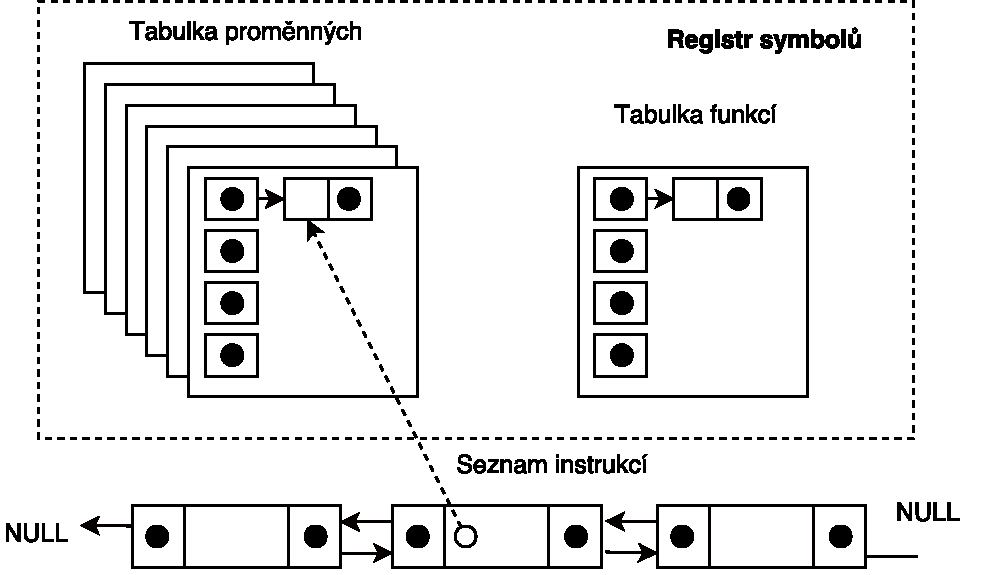
\includegraphics[width=0.6\textwidth, angle=0]{src/assets/symbol_table.pdf}
\end{figure}

Pro implementaci tabulky symbolů jsme zvolili tabulku s~rozptýlenými položkami s~použitým lineárním seznamem pro synonyma.
Tuto strukturu jsme kromě tabulek symbolů funkcí a proměnných použili ke sběru dat v~optimalizátoru cílového kódu. Bylo tedy nutné tuto strukturu implementovat vhodně tak, aby pro každé použití mohla držet různá data ve svých položkách. Existuje tedy základní verze položky \ic!SymbolTableBaseItem!, která zapouzdřuje pouze klíč a ukazatel na další položku v~lineárně svázaném seznamu synonym.

Pro konkrétní použití jsou poté vytvořeny struktury \ic|SymbolVariable| a \ic|SymbolFunction| obsahující nutná data pro tyto symboly (datový typ, rámec, úroveň zanoření resp. návratový typ, seznam parametrů) - tyto struktury obsahují obecnou \ic!SymbolTableBaseItem! vždy na prvním místě, aby bylo možné použít přetypovávání pro algoritmy. Veškeré základní operace nad tabulkou poté fungují nad \ic!SymbolTableBaseItem! pro obecnost algoritmů. Samotná tabulka také může obsahovat ukazatel na funkci, která samotnou položku inicializuje po vytvoření, resp. uvolní před smazáním.

Pro sémantické kontroly v~modulu \ic|ParserSemantic| existuje struktura \ic|SymbolRegister| zapouzdřující tabulku funkcí a zásobník tabulek proměnných. Dále obsahuje čítač pro generování unikátních identifikátorů pro symboly v~cílovém kódu. Zásobník je implementován jako jednosměrně svázaný seznam tabulek proměnných a tabulky jsou do něj vkládány/vyjímány při každé zanoření bloků jazyka IFJ17.

\subsection{Správa paměti}
Pro kontroly neuvolněných paměťových bloků dynamické správy paměti byl vytvořen modul \ic|MemoryManager|, na který je napojen pár maker \ic|memory_alloc| a \ic|memory_free|. Tato makra mají identické rozhraní s~vestavěnými funkcemi \ic|malloc| a \ic|free|, avšak zachovávají informace o~alokovaných \uv{stránkách} paměti, které se vždy uvolňují až na konci běhu programu. Stránky jsou dvousměrně svázány do seznamu pro přístup (\uv{uvoľňování}) s~časovou složitostí $\mathcal{O}(1)$.

\subsection{Optimalizace}
Z~vyšších datových struktur je zde použit \textbf{orientovaný graf a množina}. Z~těch nižších poté obecný dvousměrně svázaný seznam, zásobník implementovaný pomocí jednosměrně svázaného seznamu a tabulka s~rozptýlenými položkami. Množina je zde implementována jako dvousměrně svázaný seznam (\emph{narozdíl od doporučované varianty s~binárním stromem}) vzhledem k~očekávanému nízkému počtu položek v~ní a tím i příznivé časové složitosti $\mathcal{O}(n\cdot log(n))$. Orientovaný graf je implementován jako \textbf{jednorozměrné pole uzlů tohoto grafu} - každý uzel poté obsahuje množinu vstupních a výstupních hran pro konkrétní uzel. V~tomto grafu jsou silně propojené komponenty vyhledávány pomocí \textbf{Tarjanova algoritmu} \footnote{https://en.wikipedia.org/wiki/Tarjan\'s\_strongly\_connected\_components\_algorithm} pro vyhledávání s~časovou složitostí $\mathcal{O}(n)$.
	\section{Práce v týmu}
Náš tým se skládal ze čtyř členů, kteří byli odhodlaní začít
pracovat už od prázdnin.

Jako verzovací systém jsme použili GIT
na serveru Github z důvodů nulové ceny pro studenty a jednoduché
implementace. Pro vzájemnou komunikaci jsme zřidili kanál na komunikačním serveru
gitter do kterého jsme se přihlašovali pomocí svých github účtů. Pro rozebírání
důležitějších témat jsme použili github issues, pro neformálnější komunikaci
společnou konverzaci na serveru facebook.

Schůzky jsme organizovali každý týden a na každé si stanovili objem práce, který by měl
být hotový do konce týdne.


Jelikož byly všechny požadavky a způsob řešení znám již od počátku, zvolili jsme pro vývoj
vodopádový model.
Z počátku jsme všechny části vymýšleli společně a vše si kontrolovali,
aby později nemolo dojít k nedorozuměním. Když už byly vybudovíny principy,
na kterých budou dané moduly fungovat, došlo k rozdělení
odpovědností a každý dostal k dokončení jednu či více částí.

\subsection{Rozdělení práce}
\begin{itemize}
    \item Martin Kobelka - Vedoucí týmu, Lexikální analyzátor, syntaktický analyzátor, definice testů
    \item Tomáš Pazdiora - Syntaktická analýza výrazů, dokumentace
    \item Josef Kolář - Generátor kódu, implementace tabulky symbolů, systém rozšíření
    \item Son Hai Nguyen - Optimalizace kódu, poloautomatické generování pravidel, debuger
\end{itemize}
	\section{Závěr}
Úlohou projektu bylo především si vykoušet techniky přednášené v~předmětech IFJ a IAL prakticky,
naučit se metody výstavby překladačů, získat další znalosti z~programování v~týmu a také vzájemnou spolupráci.

Projekt byl pro nás velkou \textbf{výzvou} a svou odborností převyšoval vše, s~čím jsme do té doby měli dočinění - práce na projektu nám přinesla velké množství zkušeností.

Kromě správnosti jsme se také zaměřovali na \textbf{správnou dekompozici} problémů a snahu o~\uv{čistý} kód. Výsledný překladač je obohacen o~7 rozšíření a byl vyvíjen dle normy \emph{C11}, je tedy nezávislý na platformě. Repozitář tohoto projektu bude po domluvě zveřejněn na serveru GitHub.

\emph{
	Z~metrik projektu by bylo vhodné zmínit počet majoritních souborů, 40 .c, 40 .h a 25 .cpp jednotkových testů, celkem \emph{24805} řádků zdrojového kódu a \emph{903} commitů v~systému \emph{Git}, průměrně \emph{10} denně za aktivní dny vývoje.
}
	\newpage	
	\section{Předpřipravené ukázky}

\subsection{Pseudokod algoritmu}

\begin{algorithm}[h]
    \For{$i = 0$ \KwTo $100$}{
    print\_number = true\;
    \If{i is divisible by 3}{
    print\_number = false\;
    }
    \If{i is divisible by 5}{
    print "Buzz"\;
    }
    print a newline\;
    }
    \caption{Ukázka pseudokodu algoritmu}
\end{algorithm}

\subsection{Kod v programovacím jazyce}

\begin{lstlisting}[caption = Print arguments of command line]
#include <stdio.h>

/**
* Comments are gray but it can by styled by configure values in dokumentace.tex
*
* @param int argc Count of arguments of command line
* @param *char[] argv List of command line arguments
*/
int main(int argc, char *argv[]) {

// For cycle
for(int i = 0; i < argc; i++) {
printf("%s\n", argv[i]);
}
return 0;
}
\end{lstlisting}
\subsection{Vizualizace datových struktur}
\includesvg{src/assets/data_structure}
\end{document}